\documentclass[14pt,a4paper]{extarticle}

\usepackage[utf8]{inputenc}
\usepackage[T2A]{fontenc}
\usepackage{amssymb,amsmath,mathrsfs,amsthm}
\usepackage[russian]{babel}
\usepackage{graphicx}
\usepackage[footnotesize]{caption2}
\usepackage{indentfirst}
\usepackage{multicol}
\usepackage{listings}
\usepackage{float}
\usepackage{url}

\usepackage{enumitem}

%\usepackage[ruled,section]{algorithm}
%\usepackage[noend]{algorithmic}
%\usepackage[all]{xy}
\usepackage{booktabs}
\usepackage{graphicx}
\usepackage[table,xcdraw]{xcolor}
\usepackage{tcolorbox}

%Библиотека для блок-схем
\usepackage{tikz}
\usetikzlibrary{shapes,arrows}

% Параметры страницы
\textheight=24cm
\textwidth=16cm
\oddsidemargin=5mm
\evensidemargin=-5mm
\marginparwidth=36pt
\topmargin=-1cm
\footnotesep=3ex
%\flushbottom
\raggedbottom
\tolerance 3000
% подавить эффект "висячих стpок"
\clubpenalty=10000
\widowpenalty=10000
%\renewcommand{\baselinestretch}{1.1}
\renewcommand{\baselinestretch}{1.5} %для печати с большим интервалом

\newcommand{\angstrom}{\mbox{\normalfont\AA}}

\newtheorem{definition}{Определение} % задаём выводимое слово (для определений)
\newtheorem{example}{Замечание} % задаём выводимое слово (для определений)
\newtheorem{theorem}{Теорема} % задаём выводимое слово (для определений)
\newtheorem{construction}{Конструкция} % задаём выводимое слово (для определений)

\begin{document}
\begin{titlepage}



\begin{center}
\ \vspace{-2cm}

{МОСКОВСКИЙ ГОСУДАРСТВЕННЫЙ УНИВЕРСИТЕТ \\ ИМЕНИ М. В. ЛОМОНОСОВА}\\
{\bfseries Механико-математический факультет\\}
{Кафедра теории вероятностей}
\vspace{0.5cm}\\
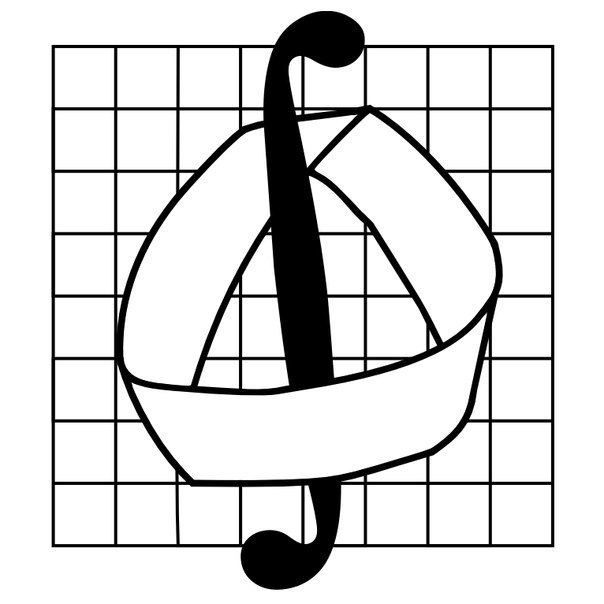
\includegraphics[width=0.2\textwidth]{emblem.jpg}\\
\vspace{1cm}

{\large Курсовая работа}\\
{\Large\bfseries
Исследование устойчивости некоторых алгоритмов отбора признаков\\}
\end{center}

\vspace{1cm}
\begin{flushright}
  \textbf{Работу выполнила:}\\ студент 408 группы\\
  Кондаурова Ксения Сергеевна\\
  \textbf{Научный руководитель:}\\
 доктор физико-математических наук
 \\профессор 
 Булинский А.В.\\
 
\end{flushright}

\vspace{3cm}
\begin{center}
Москва, 2023
\end{center}
\enlargethispage{4\baselineskip}




\newpage
\end{titlepage}
\newpage
\begin{abstract}
Курсовая работа посвящена важной задаче отбора признаков в данных большого объёма. Если говорить точнее, то рассматривается метод устойчивого выбора, который впервые был предложен в 2010 году. Он предполагает повторное применение базового алгоритма к случайным подвыборкам наблюдений или признаков, а затем отбор факторов на основе частоты их появления в проведённом эксперименте.

Вводятся все необходимые термины и подробно описывается статистическая модель, исследуемая авторами статей, на которые опирается наша работа. Также нами подробно изучены некоторые аспекты данной теории, упомянутые в нескольких работах вскользь, но имеющие принципиальное значение для понимания проблемы. 

 Удалось детально рассмотреть ряд основных известных результатов, освящённых авторами, применить знания, полученные на научных семинарах в этом году, и получить некоторое дополнение к ранее опубликованным теоремам.
\end{abstract}




\newpage
\renewcommand{\contentsname}{Содержание}
\tableofcontents




\newpage
\section{Введение}

\subsection{Задача отбора признаков}
Часто наборы данных, с которыми приходится работать, содержат большое количество признаков, число которых может достигать нескольких сотен тысяч. исследуемой проблемы.

\subsection{Устойчивость алгоритма}
Одной из важных характеристик методов отбора значимых признаков является \textit{устойчивость} -- нечувствительность алгоритма выбора признаков к небольшим возмущениям во входных обучающих данных. 


\subsection{Метод устойчивого выбора}
\textit{Метод стабильного выбора} впервые описали Meinshausen и Bühlmann в статье [2], которая сильно повлияла на дальнейшие исследования этой проблемы. 



\section{Общие сведения о методе}
\subsection{Статистическая модель}

 \begin{definition}
\textit{Процедурой выбора переменных} называется статистика $\hat{S_N} = \hat{S_N}(Z_1, ... Z_N)$, принимающая значения в $\{1, . . . , D\} $ такая, что $\hat{S_N}$ является оценкой множества сигнальных признаков $S_0$.
\end{definition}


\section{Основной результат}


\subsection{Теорема Фишера-Типпета-Гнеденко}

Теорема экстремальных типов (также известная как теорема Фишера-Типпета-Гнеденко) описывает все возможные формы распределения $M_n$ при линейной нормировке. 
\\
\\
\textbf{Теорема 1. [11]} \textit{
Пусть $X_1, X_2, ...$ -- последовательность независимых одинаково распределённых случайных величин. Если найдутся последовательности констант $c_n > 0, d_n \in \mathbb{R}, n = 1,2,...$, и невырожденная функция распределения $H$, такие что} 
\begin{center}
  $c_n^{-1}(\max(X_1,...,X_n)-d_n) \xrightarrow{d} H$,
\end{center}
\textit{то $H$ принадлежит к одному из трёх типов распределений:}
\begin{itemize}
  \item \textit{распределению Фреше: \[ \Phi_\alpha(x) =
  \begin{cases}
    0      & \quad \text{если } x \leq 0\\
    exp(-x^{-\alpha})  & \quad \text{если }  x > 0
  \end{cases}
\]}

\item \textit{распределению Вейбулла: \[ \Psi_\alpha(x) =
  \begin{cases}
    exp(-(-x)^{-\alpha})      & \quad \text{если } x \leq 0\\
    0  & \quad \text{если }  x > 0
  \end{cases}
\]}

\item \textit{распределению Гумбеля: 
$\Lambda(x) = exp(-e^{-x}), x \in \mathbb{R}$}

\end{itemize}

\textit{В таком случае говорят, что распределение $X_i$ лежит в области максимального притяжения (MDA) распреления $H$.}
\\
\\
Известны критерии, дающие необходимые и
достаточные условия принадлежности F области притяжения того или иного экстремального типа. Есть также
распределения, которые не принадлежат ни одной из трёх областей максимального притяжения, например, пуассоновское распределение. Однако для дальнейших выкладок нам понадобится лишь одна нетрудная лемма (пример 3.3.15 из [12]).
\\
\\
\textbf{Лемма. [12]} \textit{Пусть $X_1, X_2, ...$ -- последовательность независимых равномерно распределённых случайных величин на отрезке [0,1], $M_n = \max(X_1,...,X_n)$.} 

\textit{Тогда $n(M_n - 1) \xrightarrow{d} \Psi_1$, $n \rightarrow \infty$}.




\section{Вывод}

Полученный мною результат позволяет создать более полную картину влияния распределения ошибки на результат работы алгоритма стабильного выбора. Конечно, доказанное утверждение всё ещё даёт информацию лишь об одном факторе. Однако в дальнейшем я планирую развить эту теорию и выводить более общие теоремы.



\newpage

\addcontentsline{toc}{section}{\protect\numberline{}Список литературы}%
\begin{thebibliography}{3}

\bibitem{folding} Khaire, Dhanalakshmi «Stability of feature selection algorithm: A review» (2019) 

\bibitem{folding} Meinshausen, N., Bühlmann, P.: Stability selection. J. R. Stat. Soc.
72(4), 417–473 (2010)

\bibitem{folding} Beinrucker, Dogan, Blanchard  «Extensions of stability selection using subsamples of observations and covariates» (2015)

\bibitem{folding} Shah, R.D., Samworth, R.J.: Variable selection with error control:
another look at stability selection. J. R. Stat. Soc. 75(1), 55–80
(2013)

\bibitem{folding} NewTechAudit «Отбор признаков в задачах машинного обучения» (2021) https://habr.com/ru/articles/550978/

\bibitem{folding} Fleuret, F.: Fast binary feature selection with conditional mutual information. J. Mach. Learn. Res. 5, 1531–1555 (2004)

\bibitem{folding} Tibshirani, R.: Regression shrinkage and selection via the lasso. J. R. Stat. Soc. 58(1), 267–288 (1996)

\bibitem{folding} Nogueira, Brown «Measuring the Stability of Feature Selection» (2016)

\bibitem{folding} Fisher R.A., Tippet L.H.C. Limiting forms of the frequency distribution of the largest or smallest member of a sample. Proc. Cambridge Phil. Soc., 24 (1928), 180-190.


\end{thebibliography}




\end{document}
